\documentclass[]{llncs}

\usepackage{graphicx}
\usepackage{amsfonts}
\usepackage{txfonts}
\usepackage{xcolor}
\usepackage{graphbox}
%\usepackage{subcaption}


\newcommand{\red}{\color{red}}
\newcommand{\black}{\color{black}}

\newcommand{\ori}{\mathcal{O}}
\newcommand{\bond}{\mathcal{H}}

\newcommand{\pos}{\mathrm{\bf pos}}




\begin{document}

\title{ON THE POWER OF ORITATAMI SYSTEMS WITH UNARY BEAD SEQUENCE\thanks{Both authors were supported by JSPS Challenging Exploratory Research Grant no. 18K19779.}}

\titlerunning{Simple oritatami systems}

\author{Szil\'ard Zsolt Fazekas\inst{1} \and
Shinnosuke Seki\inst{2}}
%
\authorrunning{S.Z. Fazekas, S. Seki}
% First names are abbreviated in the running head.
% If there are more than two authors, 'et al.' is used.
%
\institute{Akita University, Graduate School of Engineering Science\\ \email{szilard.fazekas@ie.akita-u.ac.jp} \and The University of Electro-Communications, Graduate School of Informatics and Engineering\\ \email{s.seki@uec.ac.jp}
%\url{http://www.springer.com/gp/computer-science/lncs} \and
%ABC Institute, Rupert-Karls-University Heidelberg, Heidelberg, Germany\\
%\email{\{abc,lncs\}@uni-heidelberg.de}
}
%
\maketitle


\begin{abstract}
We investigate simple Oritatami Systems in an attempt to establish lower bounds on the size and complexity of computationally universal systems. In particular, we look at Oritatami Systems, where the folding sequence consists of a number of beads of the same type and show that under reasonable assumptions, these systems are not universal.
\end{abstract}

Transcription is the first essential step of gene expression, when DNA templates are copied into single stranded RNA by a `copy machine' called RNA polymerase. The RNA strand is synthesized letter by letter ($A\rightarrow U$, $T\rightarrow A$, $G\rightarrow C$, $C\rightarrow G$) and folds up during a process called co-transcriptional folding.

In a recent breakthrough in molecular engineering by Geary, Rothemund and Andersen~\cite{RNAorigami} the co-transcriptional folding of RNA is controlled by careful design of the DNA template. As demonstrated in laboratory, this method, called RNA Origami, makes it possible to build rectangles out of RNA strands. Geary, Meunier, Schabanel and Seki~\cite{Oritatami} proposed a mathematical model for this process, called Oritatami Systems (OS).
It has been shown~\cite{Simulator} that the model is computationally universal by simulating cyclic tag systems introduced by Matthew Cook~\cite{Cook110}. The simulation involves a very large and complex OS. One future direction of research is to find smaller universal OS.

Closely related is the question of where not to look for universal systems, i.e., what are the limitations of simple OS. When considering simple OS, there are a number of restrictions one can pose on them:
\begin{itemize}
\item bounds on the delay, the number of bead types or the arity;
\item bounds on the size of the primary structure or of the attraction rule set;
\item structural conditions on the primary structure or the attraction rule set.
\end{itemize}

Rogers and Seki~\cite{SimpleSim} showed that certain OS with small delays are not universal.

Han, Kim, Rogers and Seki\cite{SelfRemove} proved that it is possible to avoid self-attraction rules without changing the behavior of OS.

In this paper we start a new line of study which concerns the alphabet size for the primary structure, i.e., the number of bead types.
%One can show that the model is computationally universal by simulating cyclic tag systems introduced by Matthew Cook~\cite{Cook110}.

\pagebreak

\section{Oritatami Systems}
An \textbf{Oritatami System} $\ori = (B, p, \bond, \delta, \alpha)$ is composed of
\begin{enumerate}
\item a finite set $B$ of \textit{bead types},
\item a (possibly infinite) \textit{transcript} $p\in B^*\cup B^\omega$, which is a sequence of beads,
\item an \textit{attraction rule set} $\bond$, which is a symmetric relation $\bond\subseteq B^2$,
\item  a positive integer $\delta$ called the \textit{delay},
\item a positive integer $\alpha$ called the \textit{arity}.
%\item a conformation $\sigma$ called the \textit{seed}.
\end{enumerate}

Computation in OS consists of folding finite sequences of beads, each from a finite set $B$ of bead types, according to the set of attraction rules $\bond \subseteq B\times B$, on the triangular lattice graph $\mathbb{T} = (\mathbb{Z}^2,\sim)$
where $(x, y) \sim (u, v)$ if and only if $$(u, v) \in \{(x-1, y), (x+1, y), (x, y+1), (x+1, y+1), (x-1, y-1), (x, y-1)\}.$$


\noindent Sometimes we will refer to the relation above as $(x,y)$ is \textit{next to} $(u,v)$. For the illustrations, the indexing of the grid lines goes from bottom to top and from left to right, and the first coordinate refers to the horizontal axis.

A (self-avoiding) path of length $n\geq 1$ between points $(x,y)$ and $(z,t)$ is a sequence of distinct points $(x_1,y_1),\dots,(x_{n+1},y_{n+1})$ such that $(x,y)=(x_1,y_1)$, $(z,t)=(x_{n+1},y_{n+1})$ and $(x_i,y_i)\sim (x_{i+1},y_{i+1})$ for all $i\in\{1,\dots,n\}$. We denote this relation by $(x,y)\sim_n (z,t)$. This way, $\sim_1$ is $\sim$. We set $\sim_0$ to mean that the points are equal.

For a point $(x,y)$, let $N_{x,y}^d$ denote the set of points which are in a \textit{neighborhood} of size $d$ of $(x,y)$, that is,
$$N_{x,y}^d = \{ (z,t) \mid \exists n\leq d: (x,y)\sim_n (z,t) \}$$
Points $(x,y)$ and $(z,t)$ are at \textit{distance} $d\geq 0$ from each other if $(z,t)\in N_{x,y}^d\setminus N_{x,y}^{d-1}$. As we will repeatedly refer to neighborhoods in our arguments, we note that the points in $N_{x,y}^d$ form a regular hexagon centered at $(x,y)$, whose sides consist of $d$ points and the number of all points in this neighborhood is $3d^2+3d+1$.

\bigskip

A \textit{conformation} $c$ of a sequence of beads $w\in B^*$ is a path of length $n-1$ labeled by $w$ in $\mathbb{T}$, i.e., a sequence $c_1,\dots , c_n\in \mathbb{T}$ of distinct points, and a labeling $\ell: \mathbb{T}\rightarrow B$, such that $\ell(c_i)=w_i$, where $w=w_1\dots w_n$.
%\begin{itemize}
%\item $\forall i,j \in \{1,\dots, n\}$: $(x_i,y_i)=(x_j,y_j) \Rightarrow i=j$
%\item $\forall i\in \{1,\dots,n-1\}$: $(x_i,y_i)\sim (x_{i+1},y_{i+1})$
%\item $\forall i\in \{1,\dots, n\}$: $\ell(x_i,y_i)=w_i$, where $w=w_1\dots w_n$.
%\end{itemize}



The grid point occupied by bead $i$ in conformation $C$ is $\pos_C(i)=c_i$. We may omit the subscript when it is clear which conformation we refer to, or when we argue about all possible conformations.
%are pairwise distinct and labelled by the letters of $w$. A partial conformation of a sequence $w$ is a conformation of a prefix of $w$. For any partial conformation $c$ of some sequence $w$, an elongation of $c$ by $k$ beads is a partial conformation of $w$ of length $|c|+k$. We denote by $C_w$ the set of all partial conformations of $w$. We denote by $c^{\triangleright k}$ the set of all elongations by $k$ beads of a partial conformation $c$ of a sequence $w$ and by $c^{\triangleleft k}$ the singleton containing the prefix of length $|c|-k$ of $c$.
%\bigskip

Given a finite \textit{attraction rule} set $\bond\subseteq B^2$ and a conformation $c$ of a sequence $w$, a bond is a pair $(i,j)$, such that $c_i\sim c_j$ and $\ell(c_i) \bond \ell(c_j)$. The energy of a conformation $c$ of $w$, written $E(c)$, is the negation of the number of bonds within $c$: formally, $E(c) = -|\{(i, j) : c_i \sim c_j \textrm{, } j > i + 1, \textrm{ and } w_i \bond w_j \}|$.

\bigskip



The arity parameter controls the maximum number of bonds in which a given bead of a conformation can participate. For instance if $\alpha=1$, then any bead can form at most one bond, even if the attraction rule set is such that multiple neighbors could be paired with the bead. As we are embedding the conformations into $\mathbb{T}$, a bead cannot form more than $6$ bonds and that only if it is the only bead in the transcript. Similarly, $5$ bonds are only possible for the first and the last bead of a conformation, hence it generally makes sense to consider an arity parameter $\alpha\leq 4$.

In this paper we will consider OS as computing devices which start with an input conformation called the \textit{seed}, usually denoted by $\sigma$. Note that in previous papers on OS, the seed was part of the definition of the system.

The transcript folds into a conformation one bead at a time, by \textit{fixing} each bead at a point in $\mathbb{T}$. The first bead of the transcript has to be fixed next to the last bead of the seed. The position of the beads (letters of $p$) is fixed one-by-one. Suppose that beads of the seed and the first $i$ beads of the transcript have been fixed into a conformation $C_i$. Then the OS chooses among all \red TBC \black


Sometimes several conformations have the maximum number of bonds and the OS keeps track of those, while discarding the less stable ones. If more than one conformation of length $N+\delta$ has the maximum attainable number of bonds and the position of or the bonds formed by the $N+1$-th bead is not the same in all of them, then the system is nondeterministic.
In this paper we deal only with deterministic systems, and aim to show that certain simple OS are not capable of universal computation.

% so that each bead $i$, together with its $\delta-1$ successors attains a conformation which has the most bonds possible for the given $i+\delta$ long prefix of $p$.

\begin{figure}
\centering
\includegraphics[width=1\linewidth]{orisys3}
\caption{Four examples of the possible conformations (left) and the conformation with the most hydrogen bonds (1) fixes a vertex with label $C$ (right).}
\label{fig:orisys3}
\end{figure}

As a short illustration of how the model works, consider the following example (Fig.~\ref{fig:orisys3}). The OriSys is $\ori= (p, R, \delta)$, where

\begin{itemize}
\item the set of beads is $B=\{A, U, C, G\}$,
\item the transcript is $p=GCAAGCUCU$,
\item the attraction rule set is $\bond = \{A-U, C-G, G-U  \}$,
\item the delay is $\delta = 3$, and
\item the arity is $\alpha=3$.
\end{itemize}


 Suppose that the first 5 beads were fixed in place along the thick black path. At the beginning of step $N$(=5) the path is extended by one vertex labeled by the $N+\delta=8$-th letter of the primary structure (C). The position of vertices $1,\cdots, N$ is fixed ($GCAAG$) and the position of the next $\delta$ vertices is not ($CUC$). Out of all possible conformations (4 shown out of many) the not yet fixed part of the path folds up into the conformation (1) with the highest number of hydrogen-bonds (4). Bonds form according to the rules of attraction $\bond$. After the most stable conformation is found the position of vertex $N+1$ ($C$) is fixed and the next step follows.


\section{Preliminaries}
By simulating a deterministic (finite) OS with Turing machines, or indeed, with some other classical model of computation, we mean that for a suitably encoded input seed, the simulator can output the suitably encoded final conformation of the OS.

To simplify the argument, we treat the computations performed by OS as decision problems in the following sense. We can look at a deterministic Oritatami system $\ori$, with some polynomial time algorithm $\mathcal{A}_\ori$, as a computing device which takes the seed and the transcript as input and accepts the input if $\mathcal{A}_\ori$ accepts the final conformation of the OS. Assuming the existence of a polytime $\mathcal{A}_\ori$ is realistic, since if the interpretation of the output does not have to be tractable, then one can hide the real computation there.
%two dimensional array $S$ of size $w\times h$, where $w$ is the width and $h$ is the height of the final conformation of the OS. We require $S[i,j]=(n,\mathrm{prev},\mathrm{next})$

We will make repeated use of the fact that for a given delay OS can be efficiently simulated by classical algorithms, as shown in~\cite{simulation}. We present a simplified version of the argument which suffices for our results here.
\begin{theorem}
For any given $\Sigma$, $\bond$, $\delta$, $\alpha$ there exists a Turing machine with 2-dimensional tape which can simulate any OS $(\Sigma, p, \bond, \delta, \alpha)$ with any seed $\sigma$, in time $O(|\sigma|+|p|)$.
\end{theorem}
\begin{proof}
Take any step in the computation, when some $i\geq 0$ beads of the transcript have been fixed, with the last bead occupying position $(x,y)$. The delay $\delta$ is constant, and there are $|N_{x,y}^\delta|=3\delta^2+3\delta+1$ points in the neigborhood of size $\delta$. The next $\delta$ beads can only be placed within $N_{x,y}^\delta$, so the number of all possible placements (including ones which are not valid conformations) is ${|N_{x,y}^\delta|\choose \delta}\cdot \delta!\in O(1)$. For each such placement, the number of all possible bond sets formed is bounded by $2^{|N_{x,y}^\delta|\choose 2}\in O(1)$. Selecting the valid placement with the maximum number of bonds or deciding that there is no such placement, therefore, can be done in time $O(1)$.
\end{proof}

In turn, a Turing machine (TM) with two dimensional tape can be easily simulated by TM with a one dimensional tape with at most a quadratic blow up in time complexity.



\begin{corollary}
For fixed $\Sigma$, $\bond$, $\delta$, $\alpha$, the class of problems solvable by OS $(\Sigma, p, \bond, \delta, \alpha, \sigma)$ is included in $\mathrm{DTIME}((|\sigma|+|p|)^2)$.
\end{corollary}

\begin{corollary}\label{polytranscript}
Let $k$ be a non-negative number. Let $\Sigma$, $\bond$, $\delta$, $\alpha$ be fixed and the transcript length bounded polynomially by the seed length, i.e., $|p|\in O(|\sigma|^k)$. Then, the language of seeds $\sigma$ accepted by an OS $(\Sigma, p, \bond, \delta, \alpha, \sigma)$ is in $\mathrm{DTIME}(|\sigma|^{2k})$.
\end{corollary}



If the transcript length is polynomially bounded by the seed length, than the accepted language is in $\mathrm{P}$. Because of the time hierarchy theorems, we know that $\mathrm{P}\subsetneq \mathrm{EXP}$, so we can conclude that such deterministic OS are not computationally universal.


Going forward, for OS with various restrictions we will establish length bounds on the transcript $p$ in terms of $|\sigma|$, above which the OS does not behave deterministically. We also give a construction which demonstrates a lower bound for the longest transcript which can be deterministically folded by an OS with arity $1$ and delay $2$ for given input seed length.


\section{Arbitrary alphabets}
Let us first recall a result about OS with arity $1$ and delay $1$.
\begin{theorem}\cite{ARITY1D1}
For an OS with arity $1$, delay $1$ and seed length $n$, the maximum length of transcript which can be folded deterministically is $9n$.
\end{theorem}

This theorem, together with Corollary~\ref{polytranscript} means that such OS are not computationally universal.
\begin{corollary}
The languages accepted by deterministic OS with arity $1$, delay $1$ are in $\mathrm{DTIME}(n^2)$.
\end{corollary}

Keeping to arity $1$, but allowing delay $2$ increases the power of OS. We demonstrate this with an infinite family of OS, which fold deterministically a transcript of length $\frac{(n-1)^2}{4}$ when receiving a given seed of length $n$.

Consider a delay $2$, arity $1$ system with bead types $B_0$ to $B_4$ and attraction rules $\{B_1-B_1,B_2-B_2, B_3-B_3,B_4-B_4\}$. Let the seed be a conformation of a $4k+1$ long bead sequence of the form $(B_1B_0B_2B_0)^kB_0$. Bead $i$ of the seed is fixed at point $(i,0)$, for all $1\leq i\leq 4k-1$. Bead $4k$ is at $(4k-1,-1)$ and bead $4k+1$ is at $(4k,0)$.

\noindent The transcript is
\begin{center}
\begin{tabular}{llllll}
$p=$ & $(B_2B_4B_1B_3)^{k-1}$ & $B_2B_4(B_1B_4B_2B_3)^{k-1}$ & $B_1B_4(B_1B_3B_2B_4)^{k-2}$ & $B_1B_3(B_2B_3B_1B_4)^{k-2}$ & $B_2B_3$\\
     & $(B_2B_4B_1B_3)^{k-3}$ & $B_2B_4(B_1B_4B_2B_3)^{k-3}$ & $B_1B_4(B_1B_3B_2B_4)^{k-4}$ & $B_1B_3(B_2B_3B_1B_4)^{k-4}$ & $B_2B_3$\\
     & \vdots\\
     & $(B_2B_4B_1B_3)^{2}$ & $B_2B_4(B_1B_4B_2B_3)^{2}$ & $B_1B_4(B_1B_3B_2B_4)^{1}$ & $B_1B_3(B_2B_3B_1B_4)^{1}$ & $B_2B_3$\\
     & $B_2B_4B_1B_4$
\end{tabular}

\end{center}
if $k$ is odd, and
\begin{center}
\begin{tabular}{llllll}
$p=$ & $(B_2B_4B_1B_3)^{k-1}$ & $B_2B_4(B_1B_4B_2B_3)^{k-1}$ & $B_1B_4(B_1B_3B_2B_4)^{k-2}$ & $B_1B_3(B_2B_3B_1B_4)^{k-2}$ & $B_2B_3$\\
     & $(B_2B_4B_1B_3)^{k-3}$ & $B_2B_4(B_1B_4B_2B_3)^{k-3}$ & $B_1B_4(B_1B_3B_2B_4)^{k-4}$ & $B_1B_3(B_2B_3B_1B_4)^{k-4}$ & $B_2B_3$\\
     & \vdots\\
     & $(B_2B_4B_1B_3)^{2}$ & $B_2B_4(B_1B_4B_2B_3)^{2}$ & $B_1B_4$\\
     & $B_1B_3B_2B_3$
\end{tabular}

\end{center}
if $k$ is even. The length of the transcript is $4k^2$. One row of the formula above corresponds to four rows of the conformation (except for the last rows).

\begin{figure}
\centering
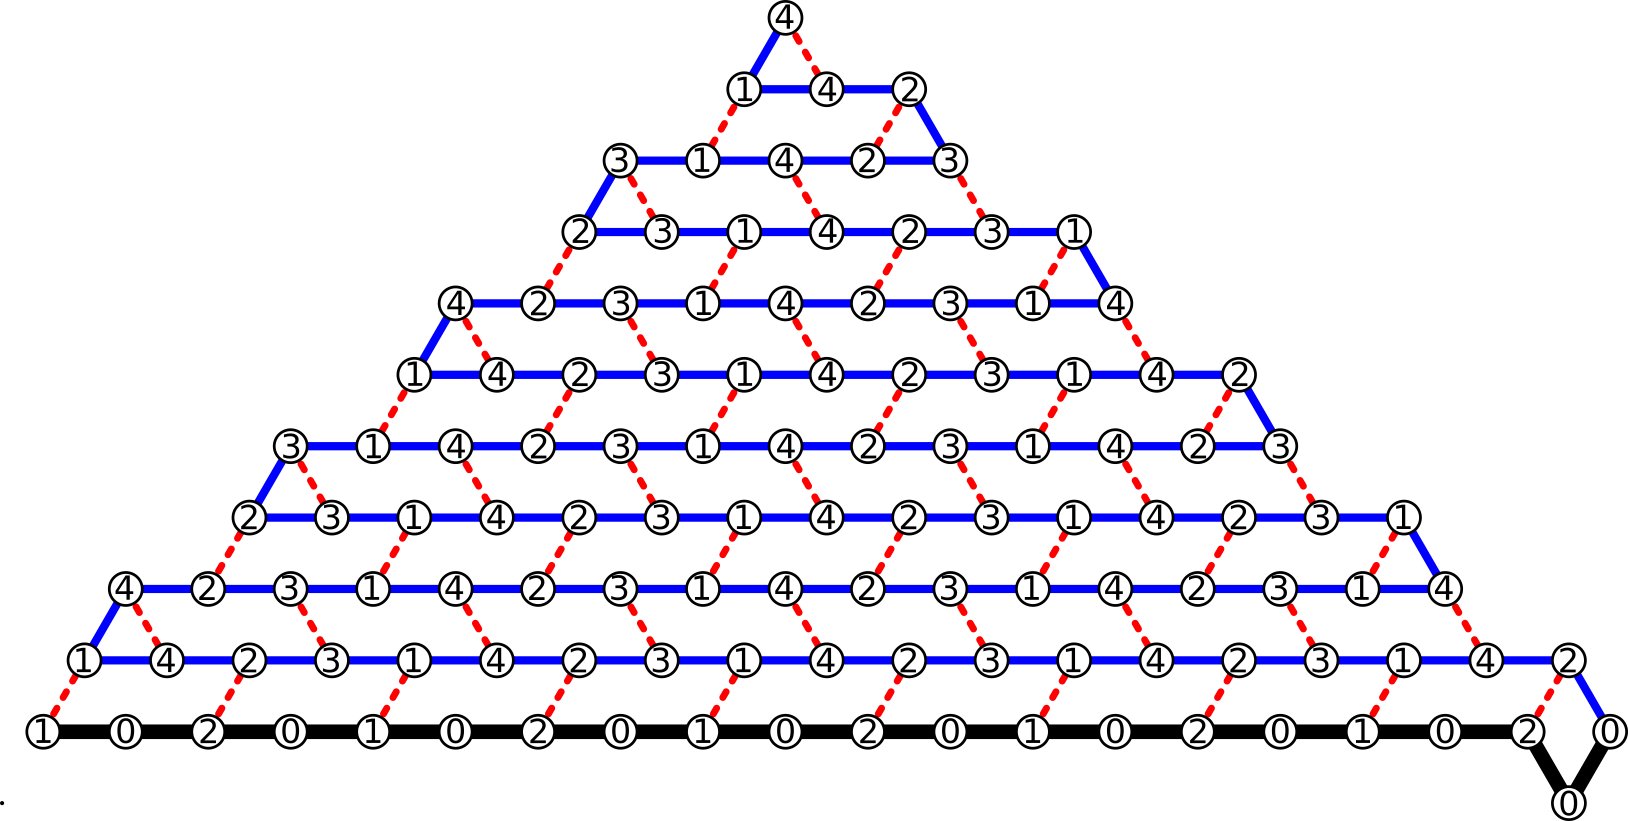
\includegraphics[width=0.9\linewidth]{./chichenBig}
\caption{Quadratic length transcript folding deterministically into pyramid shape. Seed: thick black path. Transcript: thin blue path. Bonds: dashed red lines. Beads: '$B_0$' black, '$B_1$' red, '$B_2$' red with black contour, '$B_3$' green, '$B_4$' green with black contour.}
\label{fig:chichenBig}
\end{figure}

The first bead of the transcript is type $B_2$ and it has to be fixed next to $(4k,0)$. The second bead is type $B_4$, which cannot form a bond with anything in the conformation so far. The only possibility of forming a bond is if $B_2$ is placed at $(4k,1)$ and it bonds with the $B_2$ at $(4k-1,0)$. The next bead to be fixed is $B_4$, and since it cannot form a bond, the conformation with the highest number of bonds is when the next bead, $B_1$ is at $(4k-2,1)$, which fixes the previous bead, $B_4$ at $(4k-1,1)$.



\begin{figure}
\begin{minipage}{.35\textwidth}
	\centering
	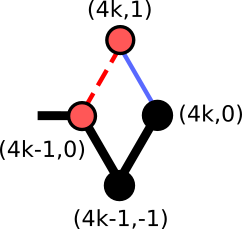
\includegraphics[align=c,height=1in]{./CI_1}\\
	\bigskip

	(a) First transcript bead
\end{minipage}%
\begin{minipage}{.2\textwidth}
	\centering
	\includegraphics[align=c,height=0.7in]{./CI_2}\\
	\bigskip

	(b) Second bead
\end{minipage}
\begin{minipage}{.4\textwidth}
	\centering
	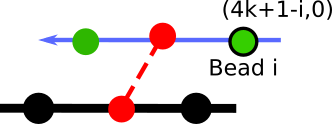
\includegraphics[align=c,height=0.5in]{./CI_3}
	\bigskip
	\vspace{0.1in}
	\includegraphics[align=c,height=0.5in]{./CI_4}
	\bigskip

	(c) Bead $i+1$, when bead $i$ is $B_{3,4}$ and $B_{1,2}$, respectively
\end{minipage}
\caption{Fixing transcript beads in odd rows}

\end{figure}


Let the last bead fixed be the $i$th one.
If it is $B_1$ or $B_2$ at some position $(4k+1-i,1)$, then the next two are $B_3B_2$ or $B_4B1$, respectively. The first beads in both cases cannot bind anywhere, whereas the second ones can bind with identical beads at $(4k+1-(i+3),0)$, fixing bead $i+1$ at $(4k+1-(i+1),1)$.
If bead $i$ was $B_3$ or $B_4$ at position $(4k+1-i,1)$ then the next two are $B_2B_4$ or $B_1B_3$,respectively. The first bead of those sequences can bind only to its identical counterpart at $(4k+1-(i+2),0)$, whereas the second cannot bind anywhere, fixing bead $i+1$ at $(4k+1-(i+1))$. The above hold as long as there is a bead already at $(4k+1-(i+3),0)$ or at $(4k+1-(i+3),0)$, respectively, so for all $i\in \{1,\dots, 4k-2\}$.

According to the above, bead $4k-1$ was fixed at $(4k+1-(4k-1),1)=(2,1)$. The next bead, $4k$ is of the same type as bead $4k-2$, so they can form a bond, and this is the only bond that can be formed by any conformation of beads $4k$ and $4k+1$ (see Fig.~\ref{fig:citurn}). A similar situation occurs when trying to fix bead $8k-2$: it can only bond to bead $8k-4$, so it will turn the path around.
\begin{figure}
	\centering
	\includegraphics[width=0.7\linewidth]{CI_turn}
	\caption{}
	\label{fig:citurn}
\end{figure}



\section{Unary}
In what follows, the alphabet of the transcript is unary, that is, there is only one bead type, say $\{A\}$. One could consider an attraction rule set where $A$ forms bonds only with beads of the seed and not with itself, but here there is only one attraction rule, $A$ binds to itself $\{A-A\}$.
Therefore, to simplify notation for unary OS we dispense with the bead alphabet and the attraction rules and we define them as $(p, \delta, \alpha)$.

We will analyze cases when the OS reaches a conformation where there is enough ``open space'', i.e., unoccupied grid points around the last fixed bead.


\subsection{Arity 1}


\paragraph{Delay 2}
Let the coordinates where the first transcript bead was fixed be $(x,y)$ and let $n=|\mathrm{seed}|+1$. We will argue about the situation when the first bead is stabilized outside $N_{x,y}^n$ (a hexagon of radius $n$). Let this be the $i$th bead of the transcript. Without loss of generality, we can translate the origin $(0,0)$ to the coordinates of bead $i-1$ (still in $N_{x,y}^n$), and we can assume that the bead outside the hexagon is fixed at $(1,1)$ (see Fig.~\ref{fig:hexagonOut}). The only position with which $(1,1)$ can form a bond is $(1,0)$. This means that there is a bead at $(1,0)$, which bonds to bead $i$, otherwise there are other conformations in which beads $i$ and $i+1$ add one bond to the conformation, making the behavior nondeterministic.

The next bead, $i+1$, can be fixed at $(2,1)$ or at $(0,1)$ as all other possibilities result in nondeterministic behavior immediately, so we have two cases.

\begin{enumerate}
\item bead $i+1$ is fixed at $(2,1)$ and can bond with a bead at $(2,0)$. Now consider bead $i+2$. For $i+1$ to be fixed at $(2,1)$, $i+2$ needs to form a bond somewhere, otherwise $i+2$ could go to $(2,1)$ forming the bond with the bead at $(2,0)$ and there would be two conformations with the maximal $1$ bond. The only possibility is that there is a bead at $(3,0)$ and $i+2$ can bond with it when placed at $(3,1)$. We can apply the same argument inductively: there is some $m\geq 0$ such that grid points $(\ell,0)$ are occupied by active beads, for all $\ell\in \{2,\dots,2+m\}$, and there is no bead at $(3+m,0)$. Such an $m$ exists, and it is not greater than $n$. Then, bead $i+\ell$ is fixed at $(\ell+1,1)$ and bonds with $(\ell+1,0)$. 
\item bead $i+1$ is fixed at $(0,1)$. This is only possible if
\begin{enumerate}
\item there is an inactive bead at $(-1,0)$ and an active one at $(-2,0)$. This case is symmetrical to (1).
\item there is no bead at $(-1,0)$, bead $i+1$ can bond with bead $i-1$ at $(0,0)$ and the bead $i+2$ can be placed at $(-1,0)$ where it can bond with $(-2,0)$, $(-2,-1)$ or $(-1,-1)$. This leads to nondeterminism, because bead $i$ at $(-1,0)$ and bead $i+1$ at $(0,1)$ has two bonds, just as the original conformation.
\item there is a bead at $(-1,0)$ and bead $i+1$ can bond with that or with bead $i-1$ at $(0,0)$. However, this means that placing bead $i$ at $(0,1)$ at bead $i+1$ at $(1,1)$ creates the same number of hydrogen bonds, thus resulting in bead $i$ not being placed deterministically.

\end{enumerate}
\end{enumerate}




\begin{figure}
\centering
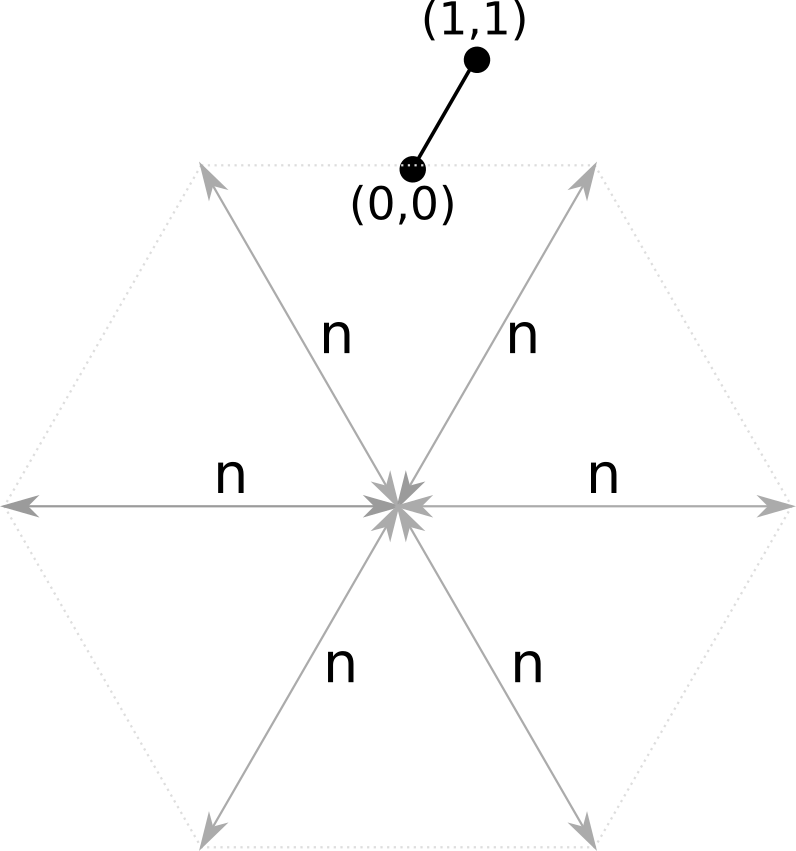
\includegraphics[width=0.3\linewidth]{./hexagonOut}
\hspace{10mm} %
\includegraphics[width=0.6\linewidth]{./hexOut}

\caption{LEFT: $N_{x,y}^n$ and the position $(1,1)$ of the first bead fixed outside of it. RIGHT: the three possible conformations with 2 bonds which would fix bead $i$ at $(1,1)$.}
\label{fig:hexagonOut}
\end{figure}




\red
At arity 1, delay 2, glider is impossible for any alphabet size
%\begin{figure}
%\centering
%\includegraphics[width=0.7\linewidth]{./IMG_20180714_113733073}
%\caption{}
%\label{fig:IMG_20180714_113733073}
%\end{figure}
%
\black
%Arity 1 delay 2:
%\begin{itemize}
%\item $m$ beads in seed
%\item $n$ transcript beads
%\item we can add 2 bonds/2 beads at most $m$ times
%\item when we first get out of the hexagon (center is the first transcript bead) of radius $m+i$, $i\geq 0$ we can only bond with transcript beads
%\item if we only add one bond/2 beads now, see figure for nondeterminism
%\item for higher delays $d$, try a similar argument, going out of a hexagon, the next $d$ beads form at most $\lfloor d/2\rfloor$ bonds, two different zigzags add enough bonds
%\end{itemize}




\section{Arity 2}
We need a lemma which gives an upper bound on the number of bonds for a (not necessarily unary) conformation of arity $2$.
\begin{lemma}
For any OS with arity $2$ and primary structure of length $n$, the maximum number of bonds is at most $n-1$.
\end{lemma}
\begin{proof}
As $\alpha=2$, if all beads realized the maximum $2$ bonds, that gives $n$ bonds, because of the handshaking lemma.

Suppose this is the case, i.e., there exists some conformation $C$ which has $n$ bonds. Consider $B$, the minimal convex bounding polygon of $C$ with all vertices in $\mathbb{T}$. Take, say, the topmost and leftmost vertex $(i,j)$ of $C$ which is on an edge of $B$. Then, $(i,j)$ being the topmost, $(i+1,x)\notin C$ for any $x$, and $(i,j)$ being the leftmost among the topmost, $(i,x)\notin C$ for any $x<j$. This excludes three neighbors of $(i,j)$ from $C$ and leaves us with the following possibilities:
\begin{enumerate}
\item $\{(i,j), (i-1,j), (i,j+1)\}\subset C$
\item $\{(i,j), (i-1,j-1), (i-1,j)\}\subset C$
\item $\{(i,j), (i-1,j-1), (i,j+1)\}\subset C$
\end{enumerate}
The first two form a sharp angle, while the third forms a wide angle. In all cases, three of the neighbors of $(i,j)$ are excluded from $C$, while two have the beads immediately preceding and succeeding the one at $(i,j)$, so there is only one neighbor left to form a bond with. This means that at least one of the beads has at most one bond, proving our claim.
\end{proof}


For arity $2$, consider an OS which can reach a conformation as shown in Fig.~\ref{fig:arity2}. Suppose the last two beads were fixed at grid points $(i-1,j-1)$ and $(i,j)$, in this order. If the following conditions hold, then the behavior of the OS is nondeterministic
\begin{itemize}
\item $\delta\geq 3$;
\item grid points $(i,j+x)$ and $(i+1,j+y)$, for all $x\in \{1,\dots,\lfloor \delta/2\rfloor\}$, $y\in \{0,\dots,\lceil\delta/2\rceil-1\}$ are not occupied;
\item the beads at $(i,j)$ and $i+1,j+1$ can both form one more bond.
\end{itemize}
Both conformations shown in the figure have the maximum $3$ bonds but the first not fixed bead has different position in the two. If the conditions above apply, the next $\delta$ beads of the primary structure can fold up into a zig-zag, adding the maximum possible $\delta$ bonds.




\begin{figure}
\centering
\includegraphics[width=0.9\linewidth]{./arity2}
\caption{Nondeterministic behavior at arity 2. The two conformations have the same number of hydrogen bonds (2 dashed lines each) and the next bead to be fixed (filled circle) occupies different grid points in the two.}
\label{fig:arity2}
\end{figure}


\paragraph{Arity 3}


\paragraph{Arity 4}



\bibliographystyle{splncs04}
\bibliography{Oritatami}

\end{document}
